\documentclass[conference]{IEEEtran}
% QONTOS Research Paper Series — Shared LaTeX Preamble
% Use with: % QONTOS Research Paper Series — Shared LaTeX Preamble
% Use with: % QONTOS Research Paper Series — Shared LaTeX Preamble
% Use with: \input{qontos-preamble}

\usepackage{cite}
\usepackage{amsmath,amssymb,amsfonts}
\usepackage{graphicx}
\usepackage{textcomp}
\usepackage{xcolor}
\usepackage{hyperref}
\usepackage{booktabs}
\usepackage{multirow}
\usepackage{array}
\usepackage{tabularx}
\usepackage{float}
\usepackage{listings}
\usepackage{url}
\usepackage{enumitem}

% Listing style
\lstset{
  basicstyle=\ttfamily\footnotesize,
  breaklines=true,
  frame=single,
  backgroundcolor=\color{gray!10},
}

% Custom column type
\newcolumntype{L}[1]{>{\raggedright\arraybackslash}p{#1}}

% QONTOS colors
\definecolor{qontosnavy}{HTML}{0A1628}
\definecolor{qontosblue}{HTML}{1E88E5}
\definecolor{qontosteal}{HTML}{00BCD4}

% Hyperref setup
\hypersetup{
  colorlinks=true,
  linkcolor=qontosblue,
  citecolor=qontosblue,
  urlcolor=qontosteal,
}

% Author block
\newcommand{\qontosauthor}{%
\IEEEauthorblockN{QONTOS Research Wing}
\IEEEauthorblockA{
Zhyra Quantum Research Institute (ZQRI)\\
Advanced Quantum Systems Division\\
Abu Dhabi, UAE\\
\texttt{research@zhyra.xyz}}
}


\usepackage{cite}
\usepackage{amsmath,amssymb,amsfonts}
\usepackage{graphicx}
\usepackage{textcomp}
\usepackage{xcolor}
\usepackage{hyperref}
\usepackage{booktabs}
\usepackage{multirow}
\usepackage{array}
\usepackage{tabularx}
\usepackage{float}
\usepackage{listings}
\usepackage{url}
\usepackage{enumitem}

% Listing style
\lstset{
  basicstyle=\ttfamily\footnotesize,
  breaklines=true,
  frame=single,
  backgroundcolor=\color{gray!10},
}

% Custom column type
\newcolumntype{L}[1]{>{\raggedright\arraybackslash}p{#1}}

% QONTOS colors
\definecolor{qontosnavy}{HTML}{0A1628}
\definecolor{qontosblue}{HTML}{1E88E5}
\definecolor{qontosteal}{HTML}{00BCD4}

% Hyperref setup
\hypersetup{
  colorlinks=true,
  linkcolor=qontosblue,
  citecolor=qontosblue,
  urlcolor=qontosteal,
}

% Author block
\newcommand{\qontosauthor}{%
\IEEEauthorblockN{QONTOS Research Wing}
\IEEEauthorblockA{
Zhyra Quantum Research Institute (ZQRI)\\
Advanced Quantum Systems Division\\
Abu Dhabi, UAE\\
\texttt{research@zhyra.xyz}}
}


\usepackage{cite}
\usepackage{amsmath,amssymb,amsfonts}
\usepackage{graphicx}
\usepackage{textcomp}
\usepackage{xcolor}
\usepackage{hyperref}
\usepackage{booktabs}
\usepackage{multirow}
\usepackage{array}
\usepackage{tabularx}
\usepackage{float}
\usepackage{listings}
\usepackage{url}
\usepackage{enumitem}

% Listing style
\lstset{
  basicstyle=\ttfamily\footnotesize,
  breaklines=true,
  frame=single,
  backgroundcolor=\color{gray!10},
}

% Custom column type
\newcolumntype{L}[1]{>{\raggedright\arraybackslash}p{#1}}

% QONTOS colors
\definecolor{qontosnavy}{HTML}{0A1628}
\definecolor{qontosblue}{HTML}{1E88E5}
\definecolor{qontosteal}{HTML}{00BCD4}

% Hyperref setup
\hypersetup{
  colorlinks=true,
  linkcolor=qontosblue,
  citecolor=qontosblue,
  urlcolor=qontosteal,
}

% Author block
\newcommand{\qontosauthor}{%
\IEEEauthorblockN{QONTOS Research Wing}
\IEEEauthorblockA{
Zhyra Quantum Research Institute (ZQRI)\\
Advanced Quantum Systems Division\\
Abu Dhabi, UAE\\
\texttt{research@zhyra.xyz}}
}


\begin{document}

\title{Gated Engineering Plan for Million-Qubit Modular Quantum Computing: A Scenario-Based Roadmap Through 2030}
\author{\qontosauthor}
\maketitle

\begin{abstract}
This capstone paper presents a gated engineering plan for the QONTOS modular quantum computing program through 2030. Rather than a single-path narrative toward one million physical qubits, we define three explicit scenarios---Base, Aggressive, and Stretch---each with measurable validation gates, quantitative no-go conditions, and concrete fallback plans. The canonical architecture proceeds through four integration levels: chiplet (approximately 2,000 qubits), module (approximately 10,000 qubits), system (approximately 100,000 qubits), and data center (approximately 1,000,000 qubits). Each level is gated by subsystem milestones in device performance, quantum error correction (QEC) overhead, photonic interconnects, cryogenic infrastructure, and classical control. We synthesize requirements from the nine preceding papers in the QONTOS series and map them onto a five-phase program with explicit decision points. Under aggressive but explicit assumptions regarding device coherence, QEC overhead reduction, and interconnect fidelity, QONTOS could reach quantum advantage on selected applications within the 2030 timeframe. The stretch scenario of 10,000 logical qubits remains a conditional north star, reachable only if every major subsystem achieves its aggressive-case milestone on schedule.

\textbf{[CLAIM-ROADMAP]} This document is a scenario-based engineering plan. All targets are conditional on stated subsystem milestones and are not unconditional predictions.
\end{abstract}

\section{Introduction and Roadmap Philosophy}

\subsection{Motivation}

The quantum computing industry has entered a phase where credible roadmaps must move beyond aspirational qubit counts toward engineering plans with explicit decision logic. IBM has published development roadmaps projecting 100,000-qubit systems through modular architectures~\cite{ibm2024}. Google Quantum AI has demonstrated error correction below the surface code threshold~\cite{google2024}. These milestones confirm that large-scale fault-tolerant quantum computing is an engineering challenge with identifiable subsystem dependencies, not a speculative ambition.

\textbf{[CLAIM-CONTEXT]} The transition from NISQ-era demonstrations~\cite{preskill2018} to fault-tolerant systems requires systematic planning with quantitative gates, not aspirational timelines.

However, as the National Academies consensus study emphasized, scaling to practical quantum advantage requires simultaneous advances across multiple subsystems---qubits, error correction, interconnects, control, and software---with failure in any single domain potentially blocking the entire program~\cite{nasem2019}. This reality demands scenario-based planning.

\subsection{Roadmap Design Principles}

This roadmap is built on four principles:

\begin{enumerate}[leftmargin=*]
\item \textbf{Scenario discipline.} Every phase specifies Base, Aggressive, and Stretch outcomes.
\item \textbf{Quantitative gates.} Advancement requires meeting measurable subsystem milestones.
\item \textbf{Explicit no-go conditions.} Each phase defines conditions under which advancement is blocked and fallback plans are activated.
\item \textbf{Cross-subsystem coordination.} A qubit milestone without a corresponding QEC or interconnect milestone does not constitute phase completion.
\end{enumerate}

\subsection{Scenario Summary}

\begin{table}[H]
\centering
\caption{Scenario summary.}
\label{tab:scenario_summary}
\begin{tabular}{@{}l L{4cm} L{3cm}@{}}
\toprule
\textbf{Scenario} & \textbf{2030 Target} & \textbf{Governing Assumption} \\
\midrule
Base & 10,000--20,000 physical qubits; 10--20 logical qubits & Current trajectories with incremental improvement \\
Aggressive & 100,000 physical qubits; 100--1,000 logical qubits & Major but plausible breakthroughs on schedule \\
Stretch & 1,000,000 physical qubits; 10,000 logical qubits & Every subsystem achieves aggressive-case milestone \\
\bottomrule
\end{tabular}
\end{table}

\textbf{[CLAIM-PROJECTION]} The Stretch scenario is not a baseline expectation. It is a conditional planning target that requires simultaneous success across all subsystem domains.

\subsection{Canonical Architecture Hierarchy}

The QONTOS architecture~\cite{qontos_p01} follows a four-level integration hierarchy:

\begin{table}[H]
\centering
\caption{Architecture integration hierarchy.}
\label{tab:arch_hierarchy}
\begin{tabular}{@{}l l l L{3cm}@{}}
\toprule
\textbf{Level} & \textbf{Name} & \textbf{Qubits} & \textbf{Challenge} \\
\midrule
L1 & Chiplet & ${\sim}2{,}000$ & On-chip wiring, yield \\
L2 & Module & ${\sim}10{,}000$ & Multi-chiplet packaging \\
L3 & System & ${\sim}100{,}000$ & Photonic links, dist.\ QEC \\
L4 & Data Center & ${\sim}1{,}000{,}000$ & Multi-fridge networking \\
\bottomrule
\end{tabular}
\end{table}

This hierarchy is consistent with modular architectures proposed by Monroe et al.~\cite{monroe2014} and reflected in IBM's modular quantum roadmap~\cite{ibm2024}.

\section{Subsystem Milestone Framework}

\begin{figure}[htbp]
\centering
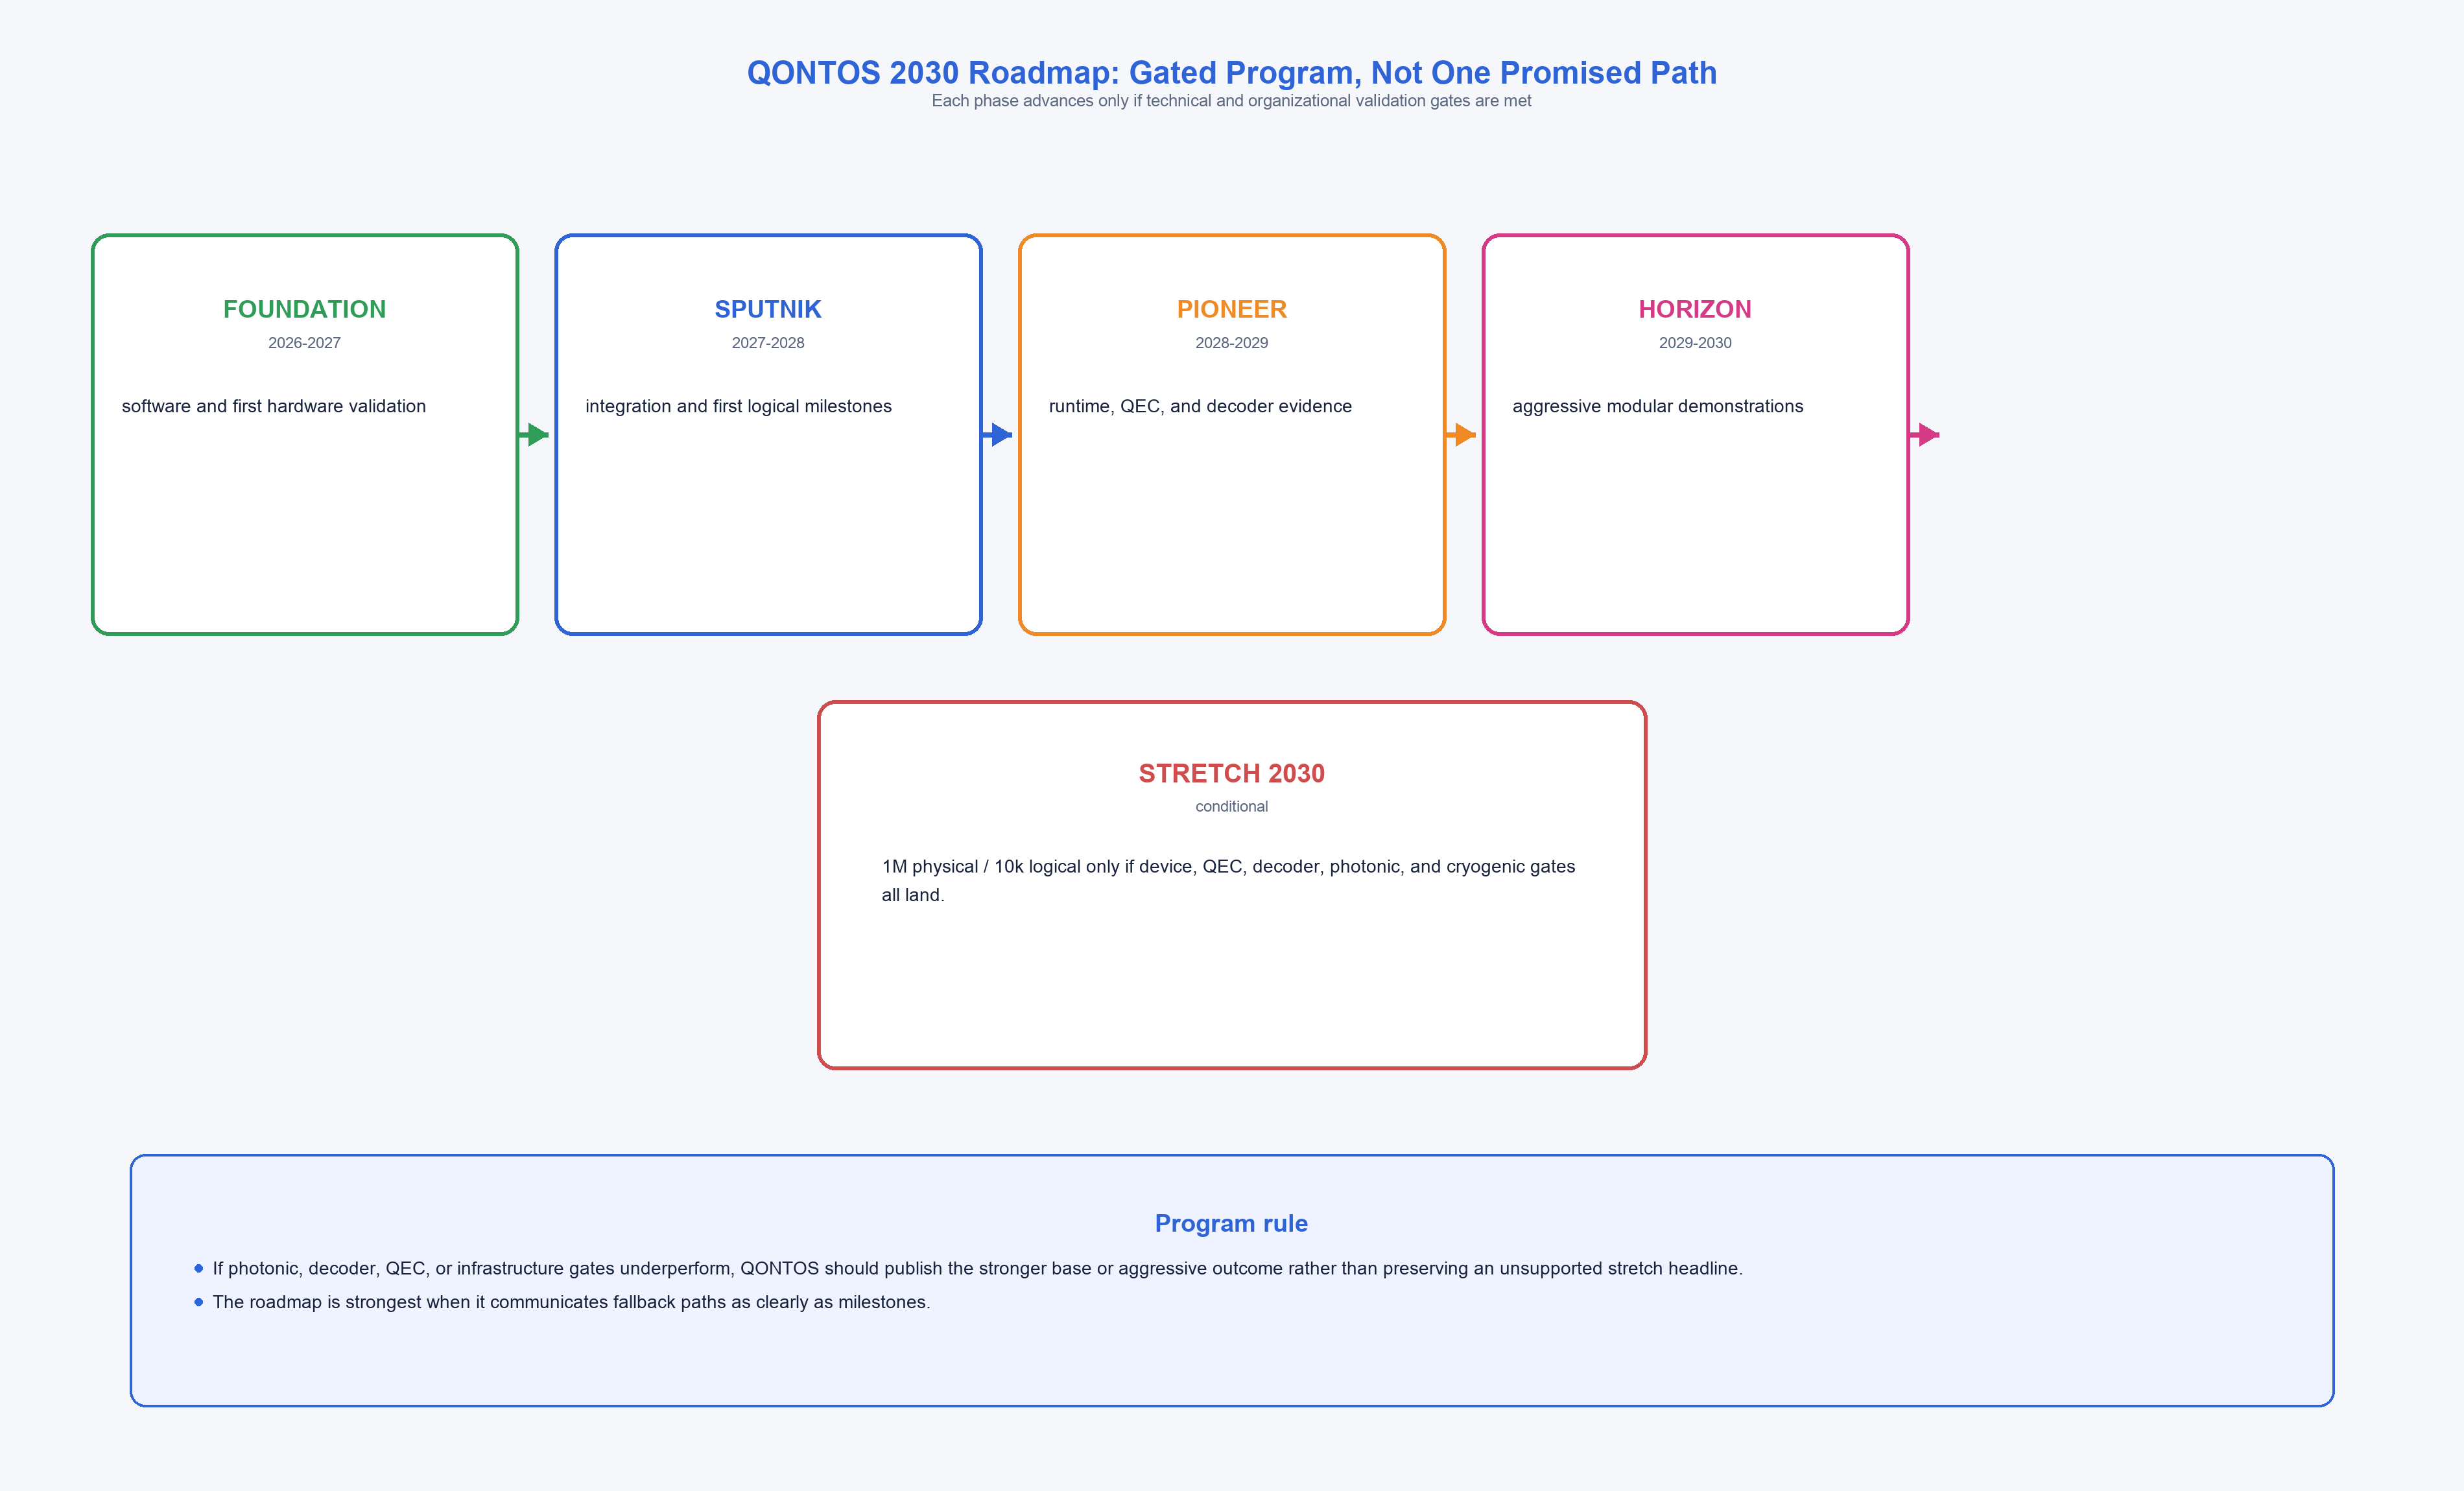
\includegraphics[width=\columnwidth]{../../figures/10_roadmap_2030.png}
\caption{Gated Development Roadmap.}
\label{fig:roadmap}
\end{figure}

Before defining program phases, we establish the subsystem milestones that gate phase transitions.

\subsection{Device Performance Milestones (from Paper~2)}

\begin{table}[H]
\centering
\caption{Device performance milestones.}
\label{tab:device_milestones}
\begin{tabular}{@{}l l l l l@{}}
\toprule
\textbf{ID} & \textbf{Metric} & \textbf{Base} & \textbf{Aggr.} & \textbf{Stretch} \\
\midrule
D-1 & $T_1$ relaxation & 300~\textmu s & 800~\textmu s & $>$1~ms \\
D-2 & $T_2$ coherence & 200~\textmu s & 500~\textmu s & $>$800~\textmu s \\
D-3 & 1Q gate error & $10^{-3}$ & $5{\times}10^{-4}$ & $10^{-4}$ \\
D-4 & 2Q gate error & $5{\times}10^{-3}$ & $10^{-3}$ & $5{\times}10^{-4}$ \\
D-5 & Chiplet yield & $>$85\% & $>$92\% & $>$96\% \\
\bottomrule
\end{tabular}
\end{table}

\textbf{[CLAIM-ENGINEERING]} Device milestones D-1 through D-4 are informed by demonstrated tantalum-on-silicon transmon performance. Kim et al.~\cite{kim2023} demonstrated utility-scale quantum computation with comparable gate fidelities.

\subsection{QEC Milestones (from Paper~3)}

\begin{table}[H]
\centering
\caption{Quantum error correction milestones.}
\label{tab:qec_milestones}
\begin{tabular}{@{}l l l l l@{}}
\toprule
\textbf{ID} & \textbf{Metric} & \textbf{Base} & \textbf{Aggr.} & \textbf{Stretch} \\
\midrule
Q-1 & QEC overhead & 1,000:1 & 300:1 & 100:1 \\
Q-2 & Logical error/round & $10^{-4}$ & $10^{-6}$ & $10^{-8}$ \\
Q-3 & Code distance & $d{=}5$ & $d{=}9$ & $d{=}13$ \\
Q-4 & Decoder latency & $<$10~\textmu s & $<$1~\textmu s & $<$500~ns \\
\bottomrule
\end{tabular}
\end{table}

\textbf{[CLAIM-ENGINEERING]} The Stretch overhead target of 100:1 is informed by Bravyi et al.~\cite{bravyi2024}. The Aggressive 300:1 target reflects surface-code implementations consistent with analyses by Chamberland et al.~\cite{chamberland2022}.

\subsection{Interconnect Milestones (from Paper~4)}

\begin{table}[H]
\centering
\caption{Interconnect milestones.}
\label{tab:interconnect_milestones}
\begin{tabular}{@{}l l l l l@{}}
\toprule
\textbf{ID} & \textbf{Metric} & \textbf{Base} & \textbf{Aggr.} & \textbf{Stretch} \\
\midrule
I-1 & Transduction eff. & $<$1\% & 5--15\% & $>$25\% \\
I-2 & Bell pair fidelity & 85\% & 95\% & $>$99\% \\
I-3 & Bell pair rate & 1~kHz & 100~kHz & $>$1~MHz \\
I-4 & Links per module & 1--2 & 4--8 & 16+ \\
\bottomrule
\end{tabular}
\end{table}

\textbf{[CLAIM-ENGINEERING]} Transduction efficiency is the single highest-risk interconnect parameter. Current laboratory demonstrations remain below 5\% end-to-end efficiency.

\subsection{Cryogenic and Control Milestones (from Papers~5 and~7)}

\begin{table}[H]
\centering
\caption{Cryogenic and control milestones.}
\label{tab:cryo_milestones}
\begin{tabular}{@{}l l l l l@{}}
\toprule
\textbf{ID} & \textbf{Metric} & \textbf{Base} & \textbf{Aggr.} & \textbf{Stretch} \\
\midrule
C-1 & Cooling at 20~mK & 20~\textmu W & 50~\textmu W & $>$100~\textmu W \\
C-2 & Control lines/module & 5,000 & 15,000 & 50,000+ \\
C-3 & Cryo mux ratio & 4:1 & 16:1 & 64:1 \\
C-4 & Power/phys.\ qubit & 50~W & 15~W & 5~W \\
\bottomrule
\end{tabular}
\end{table}

\subsection{Software and Algorithmic Milestones (from Papers~6 and~8)}

\begin{table}[H]
\centering
\caption{Software and algorithmic milestones.}
\label{tab:sw_milestones}
\begin{tabular}{@{}l l l l l@{}}
\toprule
\textbf{ID} & \textbf{Metric} & \textbf{Base} & \textbf{Aggr.} & \textbf{Stretch} \\
\midrule
S-1 & Compilation latency & $<$60~s & $<$5~s & $<$1~s \\
S-2 & Distributed overhead & $>$50\% & $<$20\% & $<$5\% \\
S-3 & Replay fidelity & 90\% & 98\% & $>$99.5\% \\
S-4 & Circuits demonstrated & Variational & FT subroutines & Full FTQC \\
\bottomrule
\end{tabular}
\end{table}

\section{Five-Phase Gated Program}

The program proceeds through five named phases, each approximately 12--18 months. Phase transitions require meeting quantitative validation gates; failure triggers explicit fallback plans.

\subsection{Phase 1: FOUNDATION (2025--2026)}

\textbf{Primary Objective:} Establish the canonical hybrid superconducting-photonic architecture, software platform, benchmarking methodology, and device characterization baseline.

\begin{table}[H]
\centering
\caption{Phase 1 scenario outcomes.}
\begin{tabular}{@{}l L{2cm} L{2cm} L{2cm}@{}}
\toprule
\textbf{Dim.} & \textbf{Base} & \textbf{Aggressive} & \textbf{Stretch Rel.} \\
\midrule
HW & Param.\ survey done; chiplet frozen & First 2k-qubit chiplet & Yield data supports L1 \\
QEC & Surface code sim.\ at $d{=}3$ & $d{=}5$ logical qubit & Overhead consistent with Q-1 \\
SW & Orchestration v1.0 & HW-in-loop sim.\ validated & DT predicts within 10\% \\
Bench. & Methodology published & Ladder through L2 & Targets set for all levels \\
\bottomrule
\end{tabular}
\end{table}

\textbf{Validation Gates:}
\begin{itemize}[leftmargin=*]
\item \textbf{GATE-F1:} Architecture constants frozen and documented.
\item \textbf{GATE-F2:} Benchmark methodology peer-reviewed and reproducible.
\item \textbf{GATE-F3:} Device assumptions populated with literature-grounded values.
\item \textbf{GATE-F4:} Software platform demonstrates end-to-end compilation and execution.
\end{itemize}

\textbf{No-Go Conditions:} No coherent benchmark program after 12 months; device literature reveals no path to D-1 Base; software cannot compile for $>$500 qubits. \textbf{Fallback:} Continue as software-first platform with external hardware partners.

\subsection{Phase 2: SPUTNIK (2026--2027)}

\textbf{Primary Objective:} Validate chiplet-to-module integration and demonstrate first logical qubits.

\begin{table}[H]
\centering
\caption{Phase 2 scenario outcomes.}
\begin{tabular}{@{}l L{2cm} L{2cm} L{2cm}@{}}
\toprule
\textbf{Dim.} & \textbf{Base} & \textbf{Aggressive} & \textbf{Stretch Rel.} \\
\midrule
HW & Multi-chiplet packaging; 5k-qubit partial & Full 10k-qubit module, $>$85\% yield & Yield supports L2 \\
QEC & $d{=}5$, overhead $<$2,000:1 & $d{=}7$, overhead ${\sim}500$:1 & Trajectory to Q-1 stretch \\
Intercon. & Intra-module coupling & First inter-module plan & Transduction 3--5\% \\
Cryo & 1 fridge, 1 module & Thermal budget for 2 modules & C-1 base met \\
\bottomrule
\end{tabular}
\end{table}

\textbf{Validation Gates:} GATE-S1 (chiplet yield $>$85\%), GATE-S2 (logical qubit lifetime $>10\times$ physical $T_1$), GATE-S3 (module thermal budget feasible), GATE-S4 (inter-module experiment design review passed).

\textbf{No-Go/Fallback:} Chiplet yield $<$80\%: pivot to smaller module topology. QEC overhead $>$3,000:1: invest in device improvement. Thermal budget exceeds capacity by $>$2$\times$: reduce module population.

\subsection{Phase 3: PIONEER (2027--2028)}

\textbf{Primary Objective:} Validate multi-module distributed execution and demonstrate fault-tolerant subroutines.

\begin{table}[H]
\centering
\caption{Phase 3 scenario outcomes.}
\begin{tabular}{@{}l L{2cm} L{2cm} L{2cm}@{}}
\toprule
\textbf{Dim.} & \textbf{Base} & \textbf{Aggressive} & \textbf{Stretch Rel.} \\
\midrule
HW & 2-module (20k Q) & 5-module (50k Q) & Path to L3 \\
QEC & Dist.\ surface code, 2 mod. & Dist.\ $d{=}9$, ${\sim}300$:1 & Q-1 stretch trajectory \\
Intercon. & Bell $>$1~kHz & Fidelity $>$93\%, $>$10~kHz & Transd.\ $>$10\% \\
SW & 2-module runtime & 5-module compiler opt. & Overhead $<$20\% \\
Algo. & Variational on logical Q & First FT subroutine & Flagship validated \\
\bottomrule
\end{tabular}
\end{table}

\textbf{Validation Gates:} GATE-P1 (Bell pair fidelity $>$85\%, rate $>$1~kHz), GATE-P2 (distributed surface code within $2\times$ single-module), GATE-P3 (decoder latency $<$10~\textmu s), GATE-P4 (at least one FT subroutine executed).

\textbf{[CLAIM-ENGINEERING]} The transduction gate is the single highest-risk decision point in the entire roadmap. If efficiency stays below 5\%, photonic multi-system networking is not viable within 2030. \textbf{Fallback:} Direct microwave inter-module coupling, limiting scale to ${\sim}50{,}000$ qubits.

\subsection{Phase 4: HORIZON (2028--2029)}

\textbf{Primary Objective:} Scale to system-level integration (100,000 qubits) and demonstrate quantum advantage on targeted applications.

\begin{table}[H]
\centering
\caption{Phase 4 scenario outcomes.}
\begin{tabular}{@{}l L{2cm} L{2cm} L{2cm}@{}}
\toprule
\textbf{Dim.} & \textbf{Base} & \textbf{Aggressive} & \textbf{Stretch Rel.} \\
\midrule
HW & 3--5 mod.\ (30--50k Q) & 10-mod.\ (100k Q) & Path to L4 \\
QEC & $\epsilon_L < 10^{-4}$ at $d{=}7$ & $\epsilon_L < 10^{-6}$ at $d{=}9$; 300:1 & On track for 100:1 \\
Intercon. & Stable $>$10~kHz & Fidelity $>$97\%, $>$100~kHz & Multi-fridge link \\
Apps. & Small mol.\ outperforms classical & Phase est.\ on relevant mol. & Resource est.\ validated \\
SW & Production orchestration & Auto partitioning $<$10\% overhead & Full-stack optimization \\
\bottomrule
\end{tabular}
\end{table}

\textbf{Validation Gates:} GATE-H1 (QEC overhead $\leq 300$:1), GATE-H2 (at least one application shows quantum advantage), GATE-H3 (multi-fridge photonic link if pursuing Stretch), GATE-H4 (monotonic benchmark improvement across three campaigns).

\textbf{[CLAIM-PROJECTION]} Reiher et al.~\cite{reiher2017} estimated that simulating the FeMoco active site requires approximately 4,000 logical qubits with T-gate counts in the billions. This remains a stretch-scenario flagship, feasible only if both QEC overhead and logical gate rates meet aggressive targets.

\subsection{Phase 5: SUMMIT (2029--2030)}

\textbf{Primary Objective:} Determine whether the Stretch architecture is reachable; deliver the strongest achievable system.

\begin{table}[H]
\centering
\caption{Phase 5 scenario outcomes.}
\begin{tabular}{@{}l L{2cm} L{2cm} L{2cm}@{}}
\toprule
\textbf{Dim.} & \textbf{Base} & \textbf{Aggressive} & \textbf{Stretch} \\
\midrule
HW & 50k Q, 5+ mod. & 100k+ Q, 10+ mod. & 1M Q, 100+ mod. \\
Logical Q & 10--50 & 100--1,000 & 10,000 \\
QEC & ${\sim}1{,}000$:1 & ${\sim}300$:1 & ${\sim}100$:1 \\
Apps. & Useful sims.; hybrid & FT on flagship & Advantage on catalysis \\
Commercial & Cloud platform & Enterprise service & Quantum data center \\
\bottomrule
\end{tabular}
\end{table}

\textbf{Validation Gates:} GATE-SM1 (device milestones at Aggressive+), GATE-SM2 (QEC overhead at target), GATE-SM3 (interconnect milestones at Aggressive+), GATE-SM4 (flagship application advantage with audit trail), GATE-SM5 ($>$168 hours continuous operation).

\textbf{Stretch-Scenario Requirements:} ALL must hold simultaneously: (1)~physical qubits $>$500,000; (2)~QEC overhead $\leq 150$:1; (3)~transduction efficiency $>$20\%; (4)~at least one application advantage that cannot be replicated classically within 1,000$\times$ the time; (5)~full software stack at data-center scale.

\textbf{[CLAIM-ROADMAP]} Failure of any single condition triggers fallback to the Aggressive architecture.

\section{Scenario Planning Tables}

\subsection{Architecture Scenario Table}

\begin{table}[H]
\centering
\caption{Architecture scenario comparison (2030).}
\label{tab:arch_scenarios}
\begin{tabular}{@{}l l l l@{}}
\toprule
\textbf{Parameter} & \textbf{Base} & \textbf{Aggr.} & \textbf{Stretch} \\
\midrule
Physical qubits & 10--20k & 100k & 1M \\
Logical qubits & 10--20 & 100--1k & 10k \\
QEC overhead & ${\sim}1{,}000$:1 & ${\sim}300$:1 & ${\sim}100$:1 \\
Arch.\ level & L2 & L3 & L4 \\
Modules & 1--2 & 10 & 100+ \\
Link type & MW direct & Photonic intra-fridge & Photonic inter-fridge \\
Fridges & 1 & 1--2 & 10+ \\
Decoder & SW MWPM & FPGA-accel. & ASIC / neural \\
Flagship & Variational & FT subroutines & Catalysis / crypt. \\
\bottomrule
\end{tabular}
\end{table}

\subsection{Investment Scenario Table}

\begin{table}[H]
\centering
\caption{Investment planning envelopes.}
\label{tab:investment}
\begin{tabular}{@{}l l l l@{}}
\toprule
\textbf{Category} & \textbf{Base} & \textbf{Aggr.} & \textbf{Stretch} \\
\midrule
Hardware R\&D & \$30--50M & \$100--150M & \$200--300M \\
Fabrication & \$10--20M & \$50--80M & \$150--200M \\
Cryogenics & \$5--10M & \$20--40M & \$80--120M \\
Software & \$15--25M & \$30--50M & \$50--80M \\
Operations & \$5--10M & \$15--25M & \$50--80M \\
\textbf{Total} & \textbf{\$65--115M} & \textbf{\$215--345M} & \textbf{\$530--780M} \\
\bottomrule
\end{tabular}
\end{table}

\textbf{[CLAIM-ESTIMATE]} Investment figures are planning envelopes informed by McKinsey's Quantum Technology Monitor~\cite{mckinsey2024} and publicly available data from comparable programs.

\subsection{Application Scenario Table}

\begin{table}[H]
\centering
\caption{Application scenario mapping.}
\label{tab:app_scenarios}
\begin{tabular}{@{}l L{1.8cm} L{2cm} L{2cm}@{}}
\toprule
\textbf{Domain} & \textbf{Base} & \textbf{Aggr.} & \textbf{Stretch} \\
\midrule
Chemistry & Small-mol.\ VQE & FT phase est. & Full FeMoco~\cite{reiher2017} \\
Materials & Variational lattice & Hubbard at scale & Correlated electrons \\
Optimization & QAOA toys & Hybrid QC opt. & Grover-accel.\ search \\
Cryptography & Shor $<$20-bit & Shor 256-bit & RSA-2048~\cite{gidney2021} \\
ML & Quantum kernels & QE feature spaces & Provable advantage \\
\bottomrule
\end{tabular}
\end{table}

\textbf{[CLAIM-CONTEXT]} Gidney and Ekera~\cite{gidney2021} estimated RSA-2048 factoring requires approximately 20 million noisy qubits, placing this firmly in the Stretch scenario. Beverland et al.~\cite{beverland2022} confirm that most applications of economic interest require $>$1,000 logical qubits.

\section{Risk Matrix}

\begin{figure}[htbp]
\centering
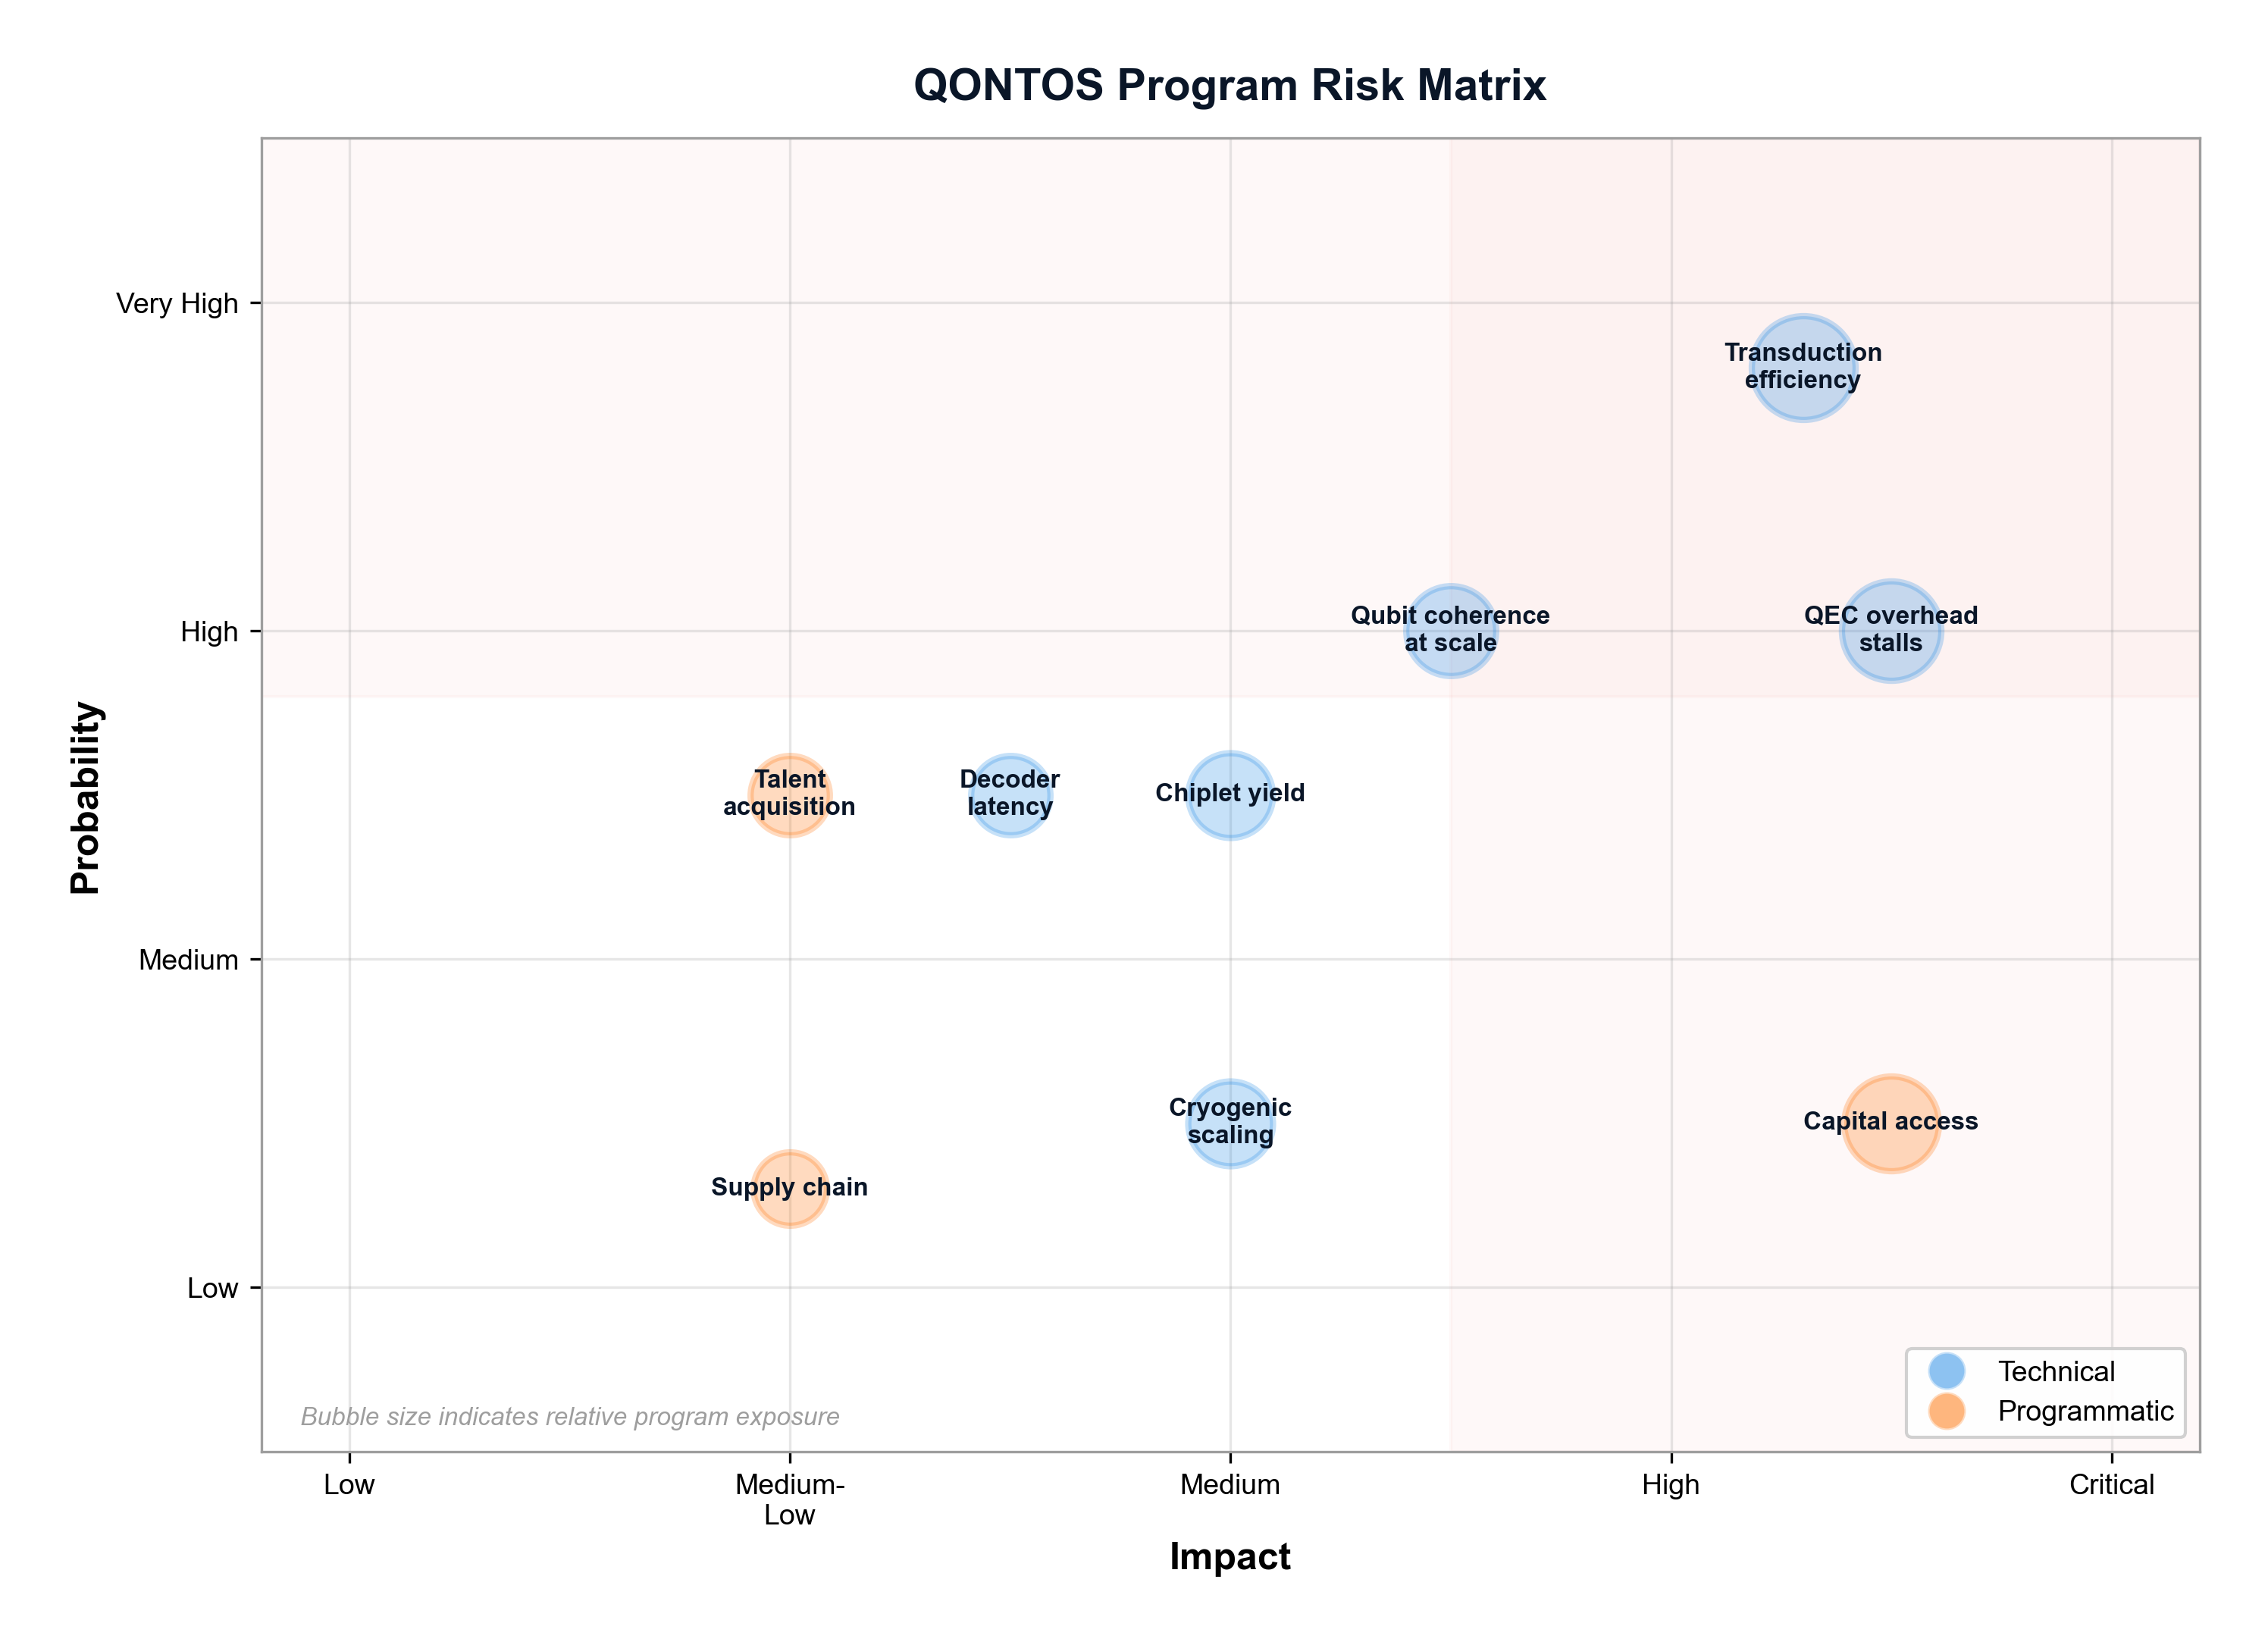
\includegraphics[width=\columnwidth]{../../figures/10_risk_matrix.png}
\caption{Program Risk Matrix.}
\label{fig:risk_matrix}
\end{figure}

\subsection{Technical Risk Assessment}

\begin{table}[H]
\centering
\caption{Technical risk assessment.}
\label{tab:tech_risk}
\begin{tabular}{@{}l L{2.5cm} l l l@{}}
\toprule
\textbf{ID} & \textbf{Risk} & \textbf{Prob.} & \textbf{Impact} & \textbf{Scenario} \\
\midrule
R-01 & Transduction plateaus $<$5\% & High & Critical & Str., Aggr. \\
R-02 & QEC overhead $>$500:1 & Med. & High & Stretch \\
R-03 & Chiplet yield $<$80\% & Med. & High & All \\
R-04 & Decoder latency too high & Med. & High & Aggr., Str. \\
R-05 & Cryo cooling insufficient & Med. & Med. & Stretch \\
R-06 & Control wiring limits & Med. & Med. & Stretch \\
R-07 & No advantage by 2029 & Med. & High & Aggr., Str. \\
R-08 & Supply chain disruption & Low & High & All \\
R-09 & Key personnel departure & Med. & Med. & All \\
R-10 & Competitor achieves first & Low & Med. & All \\
\bottomrule
\end{tabular}
\end{table}

\subsection{Programmatic Risk Assessment}

\begin{table}[H]
\centering
\caption{Programmatic risk assessment.}
\label{tab:prog_risk}
\begin{tabular}{@{}l L{3cm} l l@{}}
\toprule
\textbf{ID} & \textbf{Risk} & \textbf{Prob.} & \textbf{Impact} \\
\midrule
P-01 & Capital access interrupted & Low--Med. & Critical \\
P-02 & Fab partner constraints & Med. & High \\
P-03 & Regulatory changes & Low & Med. \\
P-04 & Timeline optimism bias & High & Med. \\
\bottomrule
\end{tabular}
\end{table}

\section{Cross-Paper Dependencies}

\subsection{Paper-to-Phase Dependency Matrix}

\begin{table}[H]
\centering
\caption{Paper-to-phase dependency matrix. C = Critical, I = Important, Inf = Informational, D = Defining, G = Governing.}
\label{tab:dependencies}
\begin{tabular}{@{}l l l l l l l@{}}
\toprule
\textbf{\#} & \textbf{Title} & \textbf{F} & \textbf{S} & \textbf{P} & \textbf{H} & \textbf{SM} \\
\midrule
1 & Architecture & C & C & I & I & I \\
2 & Ta--Si Qubits & C & C & C & I & G \\
3 & Error Corr. & I & C & C & C & G \\
4 & Photonic Links & Inf & I & C & C & G \\
5 & AI Decoding & Inf & I & I & C & C \\
6 & Software & C & C & C & C & C \\
7 & Cryo Infra. & Inf & I & I & C & C \\
8 & Algorithms & Inf & Inf & I & C & C \\
9 & Benchmarking & C & C & C & C & C \\
10 & Roadmap & D & G & G & G & D \\
\bottomrule
\end{tabular}
\end{table}

\subsection{Key Cross-Paper Dependencies}

\begin{enumerate}[leftmargin=*]
\item \textbf{Paper~2 gates Paper~3.} QEC overhead is fundamentally determined by physical error rates. If D-3 and D-4 are not met, no QEC scheme achieves targeted overhead.
\item \textbf{Paper~4 gates Paper~1 at L3+.} Without transduction milestones I-1 and I-2, the architecture cannot scale beyond L2.
\item \textbf{Paper~5 enables Paper~3 at scale.} AI-accelerated decoding is required for decoder latency at Aggressive and Stretch scales.
\item \textbf{Paper~7 constrains Paper~1.} Cryogenic cooling capacity sets hard limits on qubit density per module.
\item \textbf{Paper~9 validates all papers.} Without reproducible benchmarks, no gate can be formally passed.
\item \textbf{Paper~8 drives Paper~3 requirements.} Algorithmic resource estimates determine the QEC overhead and code distance requirements.
\end{enumerate}

\section{Integration and Decision Logic}

\subsection{Phase Transition Decision Tree}

Each phase transition follows a structured decision process: (1)~all gates met at Aggressive+ level leads to advancement on the Aggressive/Stretch track; (2)~all gates met at Base level leads to advancement on the Base track with Stretch reassessment; (3)~one or more gates failed activates fallback plans, with recovery time determining whether the phase is extended, the next phase scope is restructured, or the affected scenario is retired.

\subsection{Scenario Transition Rules}

\begin{itemize}[leftmargin=*]
\item \textbf{Stretch to Aggressive:} Triggered if any subsystem cannot demonstrate a credible path to its Stretch milestone by end of PIONEER.
\item \textbf{Aggressive to Base:} Triggered if QEC overhead remains above 500:1 at end of HORIZON, or no application benchmark shows meaningful speedup.
\item \textbf{Base is always maintained.} The program delivers commercially relevant technology under all plausible outcomes.
\end{itemize}

\subsection{Annual Review Cadence}

\begin{table}[H]
\centering
\caption{Annual review schedule.}
\begin{tabular}{@{}l l L{4cm}@{}}
\toprule
\textbf{Review} & \textbf{Timing} & \textbf{Scope} \\
\midrule
Device & Q1 & D-1--D-5; yield; fab status \\
QEC & Q2 & Q-1--Q-4; decoder dev.; code selection \\
Systems & Q3 & Integration; cryo; control scaling \\
Program & Q4 & Scenario viability; budget; go/no-go \\
\bottomrule
\end{tabular}
\end{table}

\section{Comparison with Industry Roadmaps}

\subsection{IBM Quantum Roadmap}

IBM's roadmap~\cite{ibm2024} projects 100,000-qubit systems through modular architectures. QONTOS shares the modular philosophy but differs: (a)~QONTOS targets higher qubit counts via photonic inter-refrigerator networking; (b)~QONTOS makes QEC overhead an explicit gate; (c)~QONTOS defines explicit fallback architectures at each phase.

\subsection{Google Quantum AI}

Google's demonstration of error correction below the surface code threshold~\cite{google2024} validates the surface-code approach used in the QONTOS QEC subsystem. However, Google's demonstrated system (approximately 100 physical qubits for one logical qubit) corresponds to QONTOS Phase~2, not Phase~5.

\subsection{Industry-Wide Context}

Preskill's characterization of the NISQ era~\cite{preskill2018} remains relevant. The QONTOS roadmap is designed to transition from NISQ through early fault tolerance (Base) to large-scale fault tolerance (Stretch), recognizing that most of the industry will operate in the NISQ-to-early-FT regime through 2030.

\textbf{[CLAIM-CONTEXT]} McKinsey's Quantum Technology Monitor~\cite{mckinsey2024} projects that the quantum computing market could reach tens of billions of dollars by 2040. QONTOS is positioned to contribute at any scenario level.

\section{Workforce and Organizational Requirements}

\subsection{Team Scaling by Phase}

\begin{table}[H]
\centering
\caption{Team scaling by phase.}
\label{tab:team_scaling}
\begin{tabular}{@{}l l L{4cm}@{}}
\toprule
\textbf{Phase} & \textbf{Size} & \textbf{Critical Capabilities} \\
\midrule
FOUNDATION & 30--50 & Architecture; simulation; benchmarking \\
SPUTNIK & 80--120 & Fabrication; packaging; QEC \\
PIONEER & 150--200 & Photonics; distributed systems; cryo \\
HORIZON & 250--350 & Applications; reliability; integration \\
SUMMIT & 400--500 & Operations; commercial; customer eng. \\
\bottomrule
\end{tabular}
\end{table}

\subsection{Critical Capability Gaps}

\begin{enumerate}[leftmargin=*]
\item \textbf{Microwave-to-optical transduction expertise.} Fewer than 200 researchers worldwide.
\item \textbf{Cryogenic systems engineering at scale.} Multi-refrigerator installations do not yet exist.
\item \textbf{Fault-tolerant compilation.} Must be developed in-house.
\end{enumerate}

\section{External Communication Framework}

\subsection{Communication Guardrails}

\begin{table}[H]
\centering
\caption{Communication guardrails.}
\label{tab:comm_guardrails}
\begin{tabular}{@{}l L{3.5cm} L{3.5cm}@{}}
\toprule
\textbf{Type} & \textbf{Acceptable} & \textbf{Not Acceptable} \\
\midrule
Targets & ``Our Stretch scenario targets\ldots'' & ``We will build\ldots'' \\
Timeline & ``Under aggressive assumptions, by 2030\ldots'' & ``By 2030, we will deliver\ldots'' \\
Applications & ``Our resource estimates indicate\ldots'' & ``We will achieve advantage in\ldots'' \\
Comparison & ``Our architecture shares principles with\ldots'' & ``Our approach is superior to\ldots'' \\
\bottomrule
\end{tabular}
\end{table}

\textbf{[CLAIM-ROADMAP]} All external communications must use scenario-qualified language. Unqualified claims about the Stretch scenario are not supported by this roadmap.

\section{Conclusion}

This capstone paper defines the QONTOS program as a gated engineering plan rather than a single-path promise. The five-phase structure---FOUNDATION, SPUTNIK, PIONEER, HORIZON, and SUMMIT---provides a disciplined sequence of decision points, each governed by quantitative subsystem milestones with explicit fallback plans.

The Base scenario delivers a commercially relevant modular quantum computing platform under conservative assumptions. The Aggressive scenario requires major but plausible breakthroughs consistent with current research trajectories demonstrated by Google~\cite{google2024}, IBM~\cite{ibm2024}, and leading academic groups~\cite{bravyi2024,kim2023}. The Stretch scenario of one million physical qubits and ten thousand logical qubits remains a conditional north star, achievable only if every subsystem meets its aggressive-case milestone on schedule.

Under aggressive but explicit assumptions regarding device coherence ($T_1 > 800$~\textmu s, two-qubit gate error $< 10^{-3}$), QEC overhead reduction (effective ratio below 300:1), and interconnect fidelity (transduction efficiency above 15\%, Bell pair fidelity above 97\%), QONTOS could reach quantum advantage on selected applications within the 2030 timeframe. Full-scale advantage on flagship problems such as FeMoco simulation~\cite{reiher2017} or RSA-2048 factoring~\cite{gidney2021} remains a Stretch-scenario outcome contingent on the 100:1 overhead target and data-center-scale infrastructure.

\textbf{[CLAIM-ROADMAP]} The roadmap is feasible only if it remains gated, scenario-based, and tightly linked to benchmark evidence. The stretch scenario is not a commitment; it is a conditional engineering target that defines the program's maximum ambition while the Base and Aggressive scenarios ensure that every phase delivers tangible value.

The QONTOS program, as defined in this ten-paper series, represents a comprehensive and technically grounded approach to building large-scale modular quantum computers. Its credibility rests not on the boldness of its targets but on the rigor of its gates.

\begin{thebibliography}{15}

\bibitem{ibm2024}
IBM, ``IBM Quantum Development Roadmap,'' IBM Quantum, 2024. [Online]. Available: https://www.ibm.com/quantum/roadmap

\bibitem{google2024}
Google Quantum AI, ``Quantum error correction below the surface code threshold,'' \textit{Nature}, 2024.

\bibitem{bravyi2024}
S.~Bravyi, A.~W.~Cross, J.~M.~Gambetta, D.~Maslov, P.~Rall, and T.~J.~Yoder,
``High-threshold and low-overhead fault-tolerant quantum memory,''
\textit{Nature}, vol.~627, pp.~778--782, 2024.

\bibitem{monroe2014}
C.~Monroe \textit{et al.},
``Large-scale modular quantum-computer architecture with atomic memory and photonic interconnects,''
\textit{Phys.\ Rev.\ A}, vol.~89, p.~022317, 2014.

\bibitem{reiher2017}
M.~Reiher, N.~Wiebe, K.~M.~Svore, D.~Wecker, and M.~Troyer,
``Elucidating reaction mechanisms on quantum computers,''
\textit{Proc.\ Natl.\ Acad.\ Sci.}, vol.~114, pp.~7555--7560, 2017.

\bibitem{beverland2022}
M.~E.~Beverland \textit{et al.},
``Assessing requirements to scale to practical quantum advantage,''
arXiv:2211.07629, 2022.

\bibitem{gidney2021}
C.~Gidney and M.~Ekera,
``How to factor 2048 bit RSA integers in 8 hours using 20 million noisy qubits,''
\textit{Quantum}, vol.~5, p.~433, 2021.

\bibitem{nasem2019}
National Academies of Sciences, Engineering, and Medicine,
\textit{Quantum Computing: Progress and Prospects},
The National Academies Press, Washington, DC, 2019.

\bibitem{mckinsey2024}
McKinsey \& Company, ``Quantum Technology Monitor,'' McKinsey Digital, 2024.

\bibitem{preskill2018}
J.~Preskill,
``Quantum computing in the NISQ era and beyond,''
\textit{Quantum}, vol.~2, p.~79, 2018.

\bibitem{chamberland2022}
C.~Chamberland \textit{et al.},
``Building a fault-tolerant quantum computer using concatenated cat codes,''
\textit{PRX Quantum}, vol.~3, 2022.

\bibitem{kim2023}
Y.~Kim \textit{et al.},
``Evidence for the utility of quantum computing before fault tolerance,''
\textit{Nature}, vol.~618, pp.~500--505, 2023.

\bibitem{qontos_p01}
QONTOS Research Wing,
``QONTOS Scaled Architecture for Modular Quantum Computing,''
QONTOS-ZQRI-2025-001, Paper~1 of~10.

\bibitem{qontos_p05}
QONTOS Research Wing,
``AI-Accelerated Quantum Error Decoding,''
QONTOS-ZQRI-2025-005, Paper~5 of~10.

\bibitem{qontos_p09}
QONTOS Research Wing,
``Benchmarking Methodology for Modular Quantum Systems,''
QONTOS-ZQRI-2025-009, Paper~9 of~10.

\end{thebibliography}

\end{document}
